\documentclass[a4paper,10pt]{article}
\usepackage{verbatim}
\usepackage[utf8]{inputenc}
\usepackage{graphicx}
\usepackage{caption}
\usepackage{subcaption}
\title{Analyzing Cloud Systems in Perspective of Cache Cleansing and VIrtual Switch Attack:\\
CS 6190: First Rotation Progress Report}
\author{Tanmoy Sen \\ PhD. student working as an advisee of Professor Haiying Shen\\
Email: ts5xm@virgina.edu}

\begin{document}

\maketitle

\section{Introduction}
With the advent of IoT based applications to keep every “thing” ubiquitously connected, the demand of reliable and ultra-low latency services for massive number of devices is highly increasing. Cloud infrastructure is considered to be the prime medium to provide such back-end service. In spite of its scalability, security and resource provisioning has been major issues for cloud providers that stand as obstacles to meet up their service level agreements. 

Cloud Computing has transformed the way people used to use computers. Public Infrastructure-as-a-Service (IaaS) clouds provide elastic computing and storage resources on demand. In order to maximize the resource utilization, cloud providers schedule virtual machines leased by multiple customers on same hardware resources. These resources include processors, memory systems, network resources and storage. The provider does this using virtualization where virtual machines from from multiple customers share the same physical server.

Due to its pivotal role, the resource sharing process using virtualization software  has been a prime target to the attackers. As a result, quite a few attacks targeting the virtualization layer have been formulated in the recent years. "Memory DoS" attack is an example that is reported recently. Although using VM virtualization, providers carefully isolate both physical and virtual memory pages, still most of the hardware memory-cache hierarchy is still shared by all VMs running on the same physical machine in a multi-tenant cloud environment. Consequently, a malicious VM can exploit the multi-tenancy feature to intentionally cause severe contention on the shared memory resources to conduct DoS attacks against other guest VMs sharing the resources on same physical machine.

The sharing of Last Level Cache among multiple tenants without any access control create the proper surface of such Memory Dos attacks. Zhang et al. \cite{cacheCleansing} recently proposed such a Cache Cleansing Attack that aims at causing a program from one VM to evict LLC cache lines belonging to another VM. This will increase the number of cache misses and degrade performance measure in cloud. Their case study shows that using cache cleansing attack it is possible to slow down an application running on a victim VM by up to 40 percent. They proposed a Kolmogorov Smirnov (KS) test based detection technique to this kind of memory DoS attacks. The detection scheme using KS test is not accurate for different applications. Our aim is to find a faster and multi-application detection scheme that will lead to early and accurate detection of such attacks and find a mitigation process to tackle this sort of attack.

On the other hand, with this increase in virtualization and programmability of networked systems, virtual switch has been used widely to set up the communications among the guest machines as well as with the outside network. The use of virtual switches for network virtualization makes the cloud infrastructure vulnerable to the attackers. A Return Oriented Programming(ROP) based attack has been reported recently exploiting the vulnerability of this virtual switch. In the first rotation we also aimed at to find out whether this exploit can lead to further vulnerabilities in the cloud infrastructure as a secondary objective.  

\medskip

\section{Related Works}
Many state-of-the-art works focus on network based DoS attack and resource stealing attacks in cloud platforms. Liu\cite{dos} proposed a DoS attack where an attacker can use up the victim's network bandwidth from the victim's subnet. Zhou et al.\cite{sc} designed a CPU resource attack where an attacker VM exploits the boost mechanism in the Xen credit scheduler to obtain extra resources than he paid for in the cloud. Further studies are also been done in the field of hardware resource contention. Grunwald and Ghasi\cite{grun} reflected the effect trace  cache evictions on the victim's execution platform with hyper threading enabled in specific type of processor. Based on the mentioned works, Zhang et al.\cite{cacheCleansing} first proposed Memory DoS attacks caused by contention for hardware memory resources in the cloud computing platform. In perspective of cloud computing, these availability breaches are serious security threats as they occur despite the provision memory isolation imposed by virtualization. They demonstrated co-location of only a few hostile VM can cause significant performance degradation for a distributed application. They formulated a detection technique for these memory DoS attacks, using a statistical metric on performance counter measurements. 

In the past, various attacks on cloud systems exploiting the network vulnerability of the residing VMs have been proposed. Virtual switches are a crucial component of cloud operating systems to interconnect virtual machines in a flexible manner. Thimmaraju et al.\cite{thim} first presented the systematic study of the security implications of virtual switches and identify the fundamental design challenges which make them susceptible to attacks and elevate the impact of frequently occurring vulnerabilities. Our work aims at finding vulnerabilities by exploiting the mentioned attack in \cite{thim}.  


\medskip

\section{Threat and Attack Model}

\subsection{Cache Cleansing Attack}
For launching the cache cleansing attack, we assume the adversary has the capability to launch at least one VM on the server the victim VMs are running. This model is proposed previously in order to confirm an attacker can run any program in his own VM so that he can exploit the vulnerability of resource sharing in case of multi-tenancy. Any provision of attacks launched by the cloud providers is out of the scope in case of this attack.

We assume the hardware and software isolation mechanism function correctly as designed. A hypervisor virtualizes and manages the hardware resources. Each VM is assigned a disjoint set of vCPUs which can be scheduled to operate on any physical cores based on hypervisor's scheduling algorithms. A program running on a vCPU can access the hardware resources available to the physical resources it is running on which includes the Last Level Cache (LLC).

An LLC that is shared by all cores in one socket Intel LLCs usually adopt an inclusive cache policy. According to the policy, LLCs are divided into multiple slices and each slice is associated with one physical core, although every core may utilize the entire LLC. This allows sharing of LLC by all cores inhibiting in the same socket. Consequently, a program from one core or VM can try to evict LLC cache that belongs to another core or VM. To cause LLC contention, the adversary can allocate a memory buffer to cover the entire LLC. Then by accessing one memory address per memory block in the buffer, the adversary can cleanse the entire cache and evict all of the victim's data. The objective of Cache Cleansing attacks is to repeat such a process without pauses.

\subsection{Virtual Switch Attack}
In our scenario, the attacker's target is the cloud infrastructure that uses virtual switches for network virtualization. For this purpose, we assume that our attacker only has limited access in the cloud by either renting or compromising a VM by web-application vulnerability. Based on the previous analysis, it can be conjectured that current virtual switch implementations are unstable against different attacks. One such vulnerability is a stack buffer overflow attack can be launched while parsing the MPLS packets. The stack buffer overflow occurs when a large MPLS label stack that exceeds a pre-defined threshold is parsed.

The proposed attack model by Thimmaraju et al. focuses on exploiting the stack buffer overflow vulnerability. For this purpose, a remote code execution exploit process is used by creating a ROP attack hidden in an MPLS packet. ROP uses a sequence of gadgets that facilitate the execution of desired code. Given a stack buffer overflow, the attacker overwrites the stack frame with such a ROP chain(sequence of gadgets). Ultimately, it may lead to implementation of a worm leading to compromise of the host operating system.

\medskip

\section{Detection Techniques for Cache Cleansing Attack}
\label{sec:det}
Zhang et al.\cite{cacheCleansing} hypothesize that the access characteristics to any memory resources ( cache miss rate, access rate, etc.) by a computer program or a phase of a computer program tends to follow a certain probability distribution. It is expected that this probability distribution will be changed when a memory DoS attack like cache cleansing attack occurs. They propose Kolmogorov-Smirnov (KS) test to differentiate between with attack and without attack scenario. 

For the detection purpose, we tried to use the plotting sliding window on time series data of both cache miss and cache hit ratio along side the value of KS test. 
\begin{itemize}
\item On a single run collect half of the samples without attack and rest of the samples with attack running
\item On a single run collect data with interleaving without attack and with attack phase.
\end{itemize}

As cache cleansing attack requires repeating the eviction as a continuous process, so the second method mentioned above does not provide significant output. We also tried to formulate a detection process depending on the Pearson-correlation within the data collection window.
\medskip

\section{Attack Plan on Virtual Switch}
The first phase of the attack on the virtual switch is to implement the process proposed in cite. Based on the stack buffer overflow attack, using ROP chain we have already managed to execute the dump command for the open flow table. We plan to formulate a communication graph among the nodes including the VMs communicating through a specific virtual switch which may lead to formalizing the complete network.

\medskip

\section{Results}
We have run all our experiments on our local cluster. We have created two victim VMs and one attacker VM for the purpose. The attacker VM was allocated 4 vCPUs where each victim VM was allocated 12 vCPUs. The data were sampled at a rate of 0.01 using the methods mentioned in section ~\ref{sec:det}. While the attack program was running on the attacker VM, one victim VM was running the desired application and another victim was running normal Linux processes. The data were collected by the host using Intel PCM.
\subsection{Cache Cleansing Attack}
The implemented attack is launched on different type of applications to find whether any significant pattern be identified that can distinguish the cleansing attack from regular contention period by real-time profiling of applications running on single or multiple VMs in both attack and regular scenario. Although, the proposed attack claims slowdown of an application upto 40\% our implemented attack showed slowdown in application up to only 23\%. Table 1 summarizes the application run on the victim VMs along side their execution time in both without and with attack scenario.

\begin{table}[h!]
\label{table:summary}
\caption{Application Summary}
\begin{tabular}{ |p{3.5cm}||p{3.5cm}|p{3.5cm}|}
 \hline
 \multicolumn{3}{|c|}{Application List} \\
 \hline
 Type of Application & Name of Application & Percentage of slow down \\
 \hline
 CPU Intensive	& PI & 16.78\\
 \hline
 Data Intensive & Terasort & 22.37 \\
 \hline
 Deep Learning	& Facenet	& 22.81	\\
 \hline
 Database & Hive Queries & 17.24  \\
 \hline
 Cryptography &	SHA	&  19.56 \\
  \hline
 \end{tabular}
 \end{table}
 
As expected, cache cleansing attack shows better performance against the applications those are data intensive and requires higher amount of cache accesses. As a result, Terasort and Facenet displays higher amount of slowdown with respect to the other applications. 

For the cache cleansing attack, we plan to detect the change of pattern on the basis of running average on time series data of cache miss and cache hit rate while running an application in without attack and with attack phase sequentially. Again, for terasort and facenet the change of pattern is quite evident between  without and with attack phases. But, for other applications it seems difficult to tell on the basis of time series data. 

Figure ~\ref{fig:test} shows the plot of LLC misses and LLC hit for the application terasort. In the figure, out of 8000 samples first 4000 samples are collected in absence of any attack and rest of the samples are collected after launching the attack. From the figure it is evident that the two scenarios generate different patterns in terms of amplitude.  

\begin{figure}[htb]
\centering
\begin{subfigure}{.5\textwidth}
  \centering
  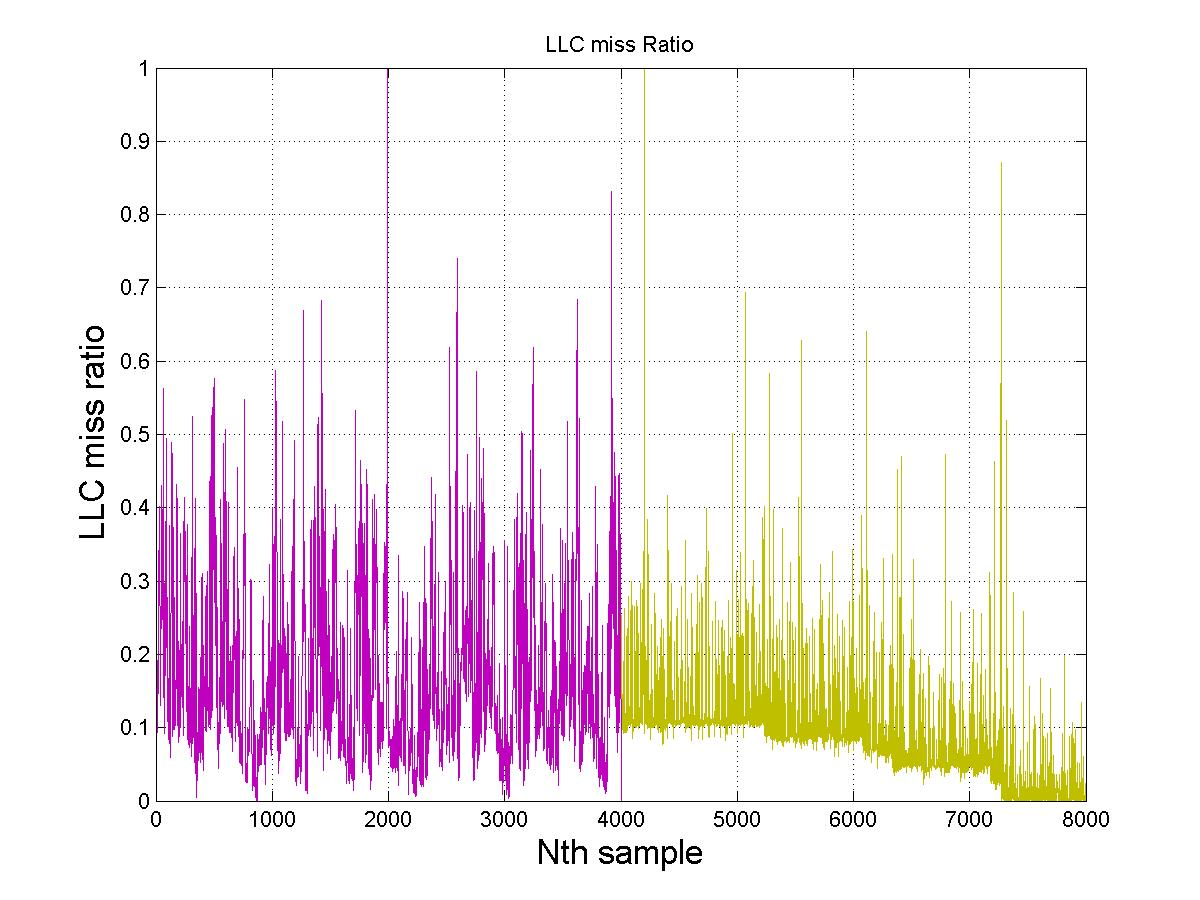
\includegraphics[width=.9\linewidth]{Figures/fig1.jpg}
  \caption{Miss Ratio}
  \label{fig:sub1}
\end{subfigure}%
\begin{subfigure}{.5\textwidth}
  \centering
  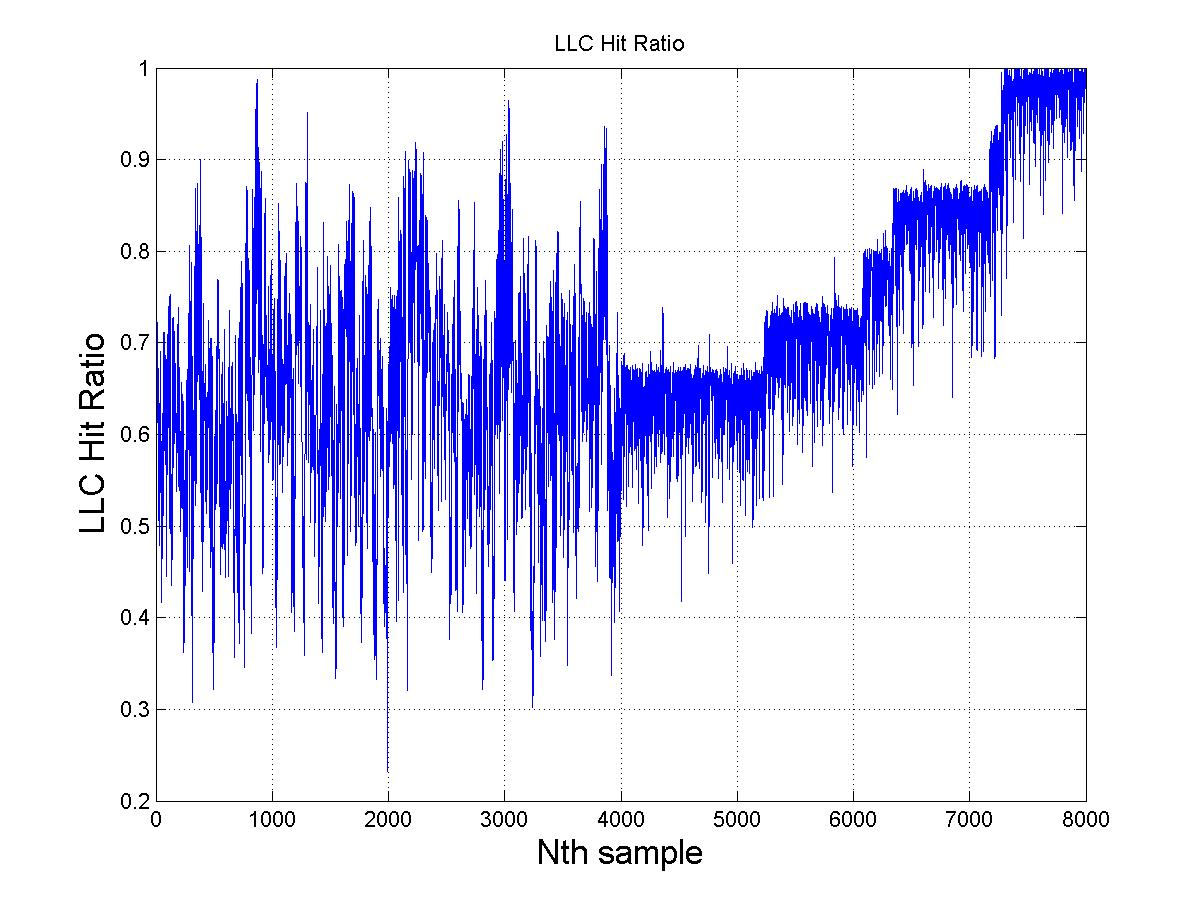
\includegraphics[width=.9\linewidth]{Figures/fig12.jpg}
  \caption{Hit Ratio}
  \label{fig:sub2}
\end{subfigure}
\caption{Output of Terasort for continuous attack and non-attack period}
\label{fig:test}
\end{figure}


\begin{figure}[htb]
\centering
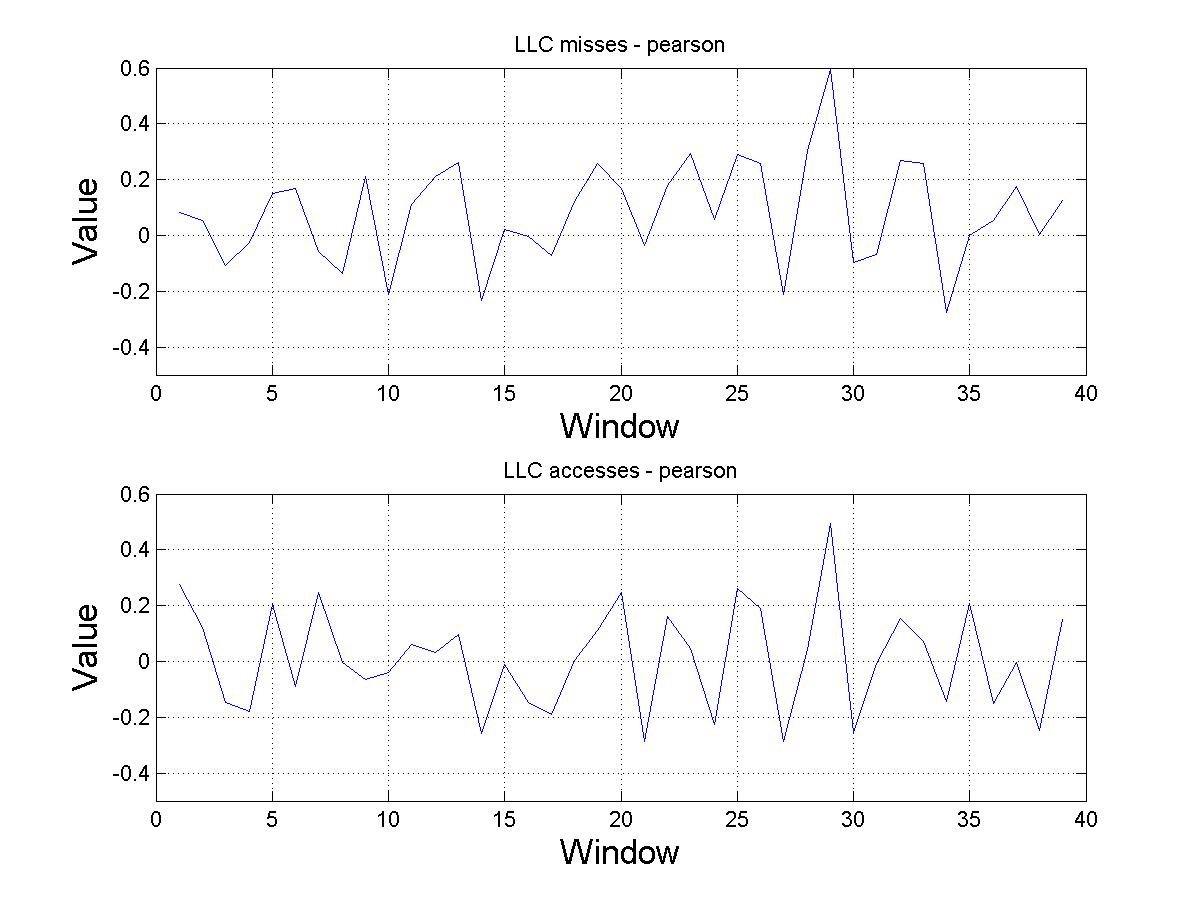
\includegraphics[width=0.6\textwidth]{Figures/fig7.jpg}
\caption{Pearson correlation}
\label{fig:pc}
\end{figure}

\begin{figure}[htb]
\centering
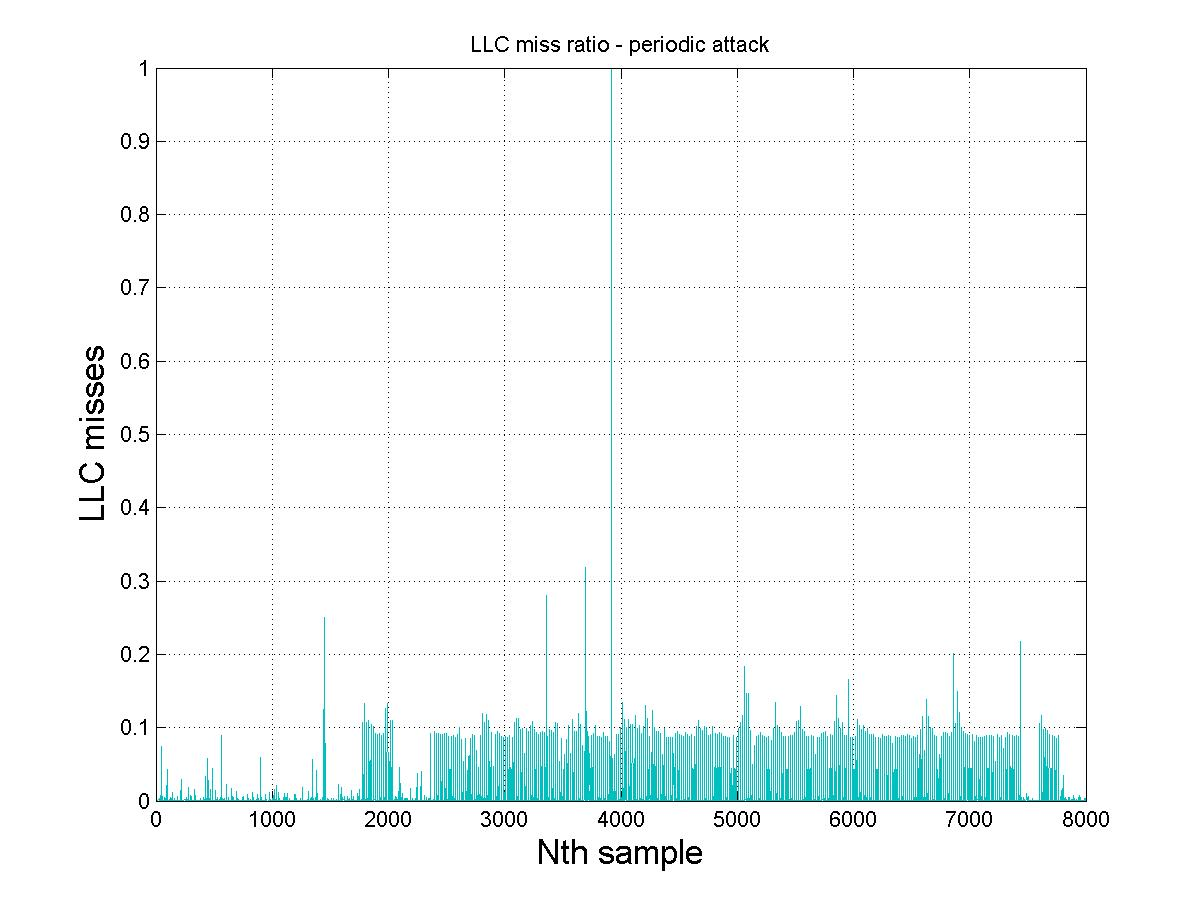
\includegraphics[width=0.6\textwidth]{Figures/fig3.jpg}
\caption{Miss ratio for interleaving attack and non-attack period}
\label{fig:il}
\end{figure}

Figure ~\ref{fig:pc} shows the pearson correlation of absolute value of LLC misses and accesses for the above mentioned scenario. But this correlation does not show any conclusive result for all the applications. On the Figure ~\ref{fig:il} shows the plot of hit rate for running the attack in an interleaving sequence. Because the cache cleansing attack demands continuous eviction of victim's cache line the data does not reflect much significant difference.  


\subsection{Virtual Switch Attack}
In terms of virtual switch attack, buffer overflow attack has been launched to execute the dump command of the flow table where only the default flow has been generated. But, while launching the attack issues related to Adress Space Layout Randomization(ASLR) is faced. If the stack protection and ASLR is triggered off then it is believed that the attack procedure can bring out significant result. 
\medskip

\section{Conclusion and Future Works}
The advancement of “Internet of Things" has resulted in a significant increase of cloud enabled devices which ultimately leads to extensive use of cloud based systems. In order to maintain the reliable service of cloud infrastructure to IoT platforms further research in its security and resource management is of prime concern. As a result, recently proposed both cache cleansing and virtual switch attack requires further investigation regarding vulnerability they may impose on the cloud platform. In future for cache cleansing attack, we need to improvise on faster and effective detection method covering different types of applications along side finding optimal defense mechanism for this attack. On the other hand, in terms of virtual switch attack, possibility of formulating the communication graph among the nodes inside the cloud platform using the gathered dump need to be analyzed. 


\begin{thebibliography}{9}
\bibitem{cacheCleansing}Tianwei Zhang, Yinqian Zhang and Ruby B. Lee,  \textit{DoS Attacks on Your Memory in Cloud}. Proceedings of the 2017 ACM on Asia Conference on Computer and Communications Security, ASIA CCS '17.
\bibitem{noHype} Rexford, Eric Keller Jakub Szefer Jennifer, and Ruby B. Lee. "NoHype: Virtualized Cloud Infrastructure without the Virtualization." Princeton University, Saint-Malo, France, ISCA 10 (2010): 19-23.
\bibitem{dos} F. Liu. "A new form of DoS attack in cloud and its avoidance mechanism" In ACM Workshop on Cloud Computing Security, 2010.
\bibitem{sc} F. Zhou, M. Goel, P. Desnoyers, and R. Sundaram. "Scheduler vulnerabilities and coordinated attacks in cloud computing." In IEEE Intl. Symp. on Network Computing and Applications, 2011.
\bibitem{grun} D. Grunwald and S. Ghiasi. "Microarchitectural denial
of service:  Insuring microarchitectural fairness." In ACM/IEEE Intl. Symp. on Microarchitecture, 2002.
\bibitem{thim} Kashyap Thimmaraju,
               Bhargava Shastry,
               Tobias Fiebig,
               Felicitas Hetzelt,
               Jean{-}Pierre Seifert,
               Anja Feldmann and
               Stefan Schmid. "Reigns to the Cloud: Compromising Cloud Systems via the Data Plane." CoRR, 2016.
\end{thebibliography}
\end{document}
